\documentclass{beamer}

\usepackage[utf8]{inputenc}
\usepackage[spanish]{babel}
\usepackage{times}
\usepackage{graphicx}
\usepackage{amsmath}
\usepackage{amsthm}
\usepackage{amssymb}

\spanishdecimal{.}

\mode<presentation> {
  \usetheme{Madrid}
  \setbeamercovered{transparent}
}

\title[Redes neuronales] %
{¿Que son las redes neuronales? \\Una introducción informal}

\author[Waissman]{Julio Waissman Vilanova}

\institute[UNISON/LCC] %
{ Licenciatura en Ciencias de la Computación\\
  Departamento de Matem\'aticas\\
  \textbf{Universidad de Sonora}
}

\date{}

\subject{Neural Network}

\begin{document}


\begin{frame}
  \titlepage
\end{frame}

\begin{frame}
  \frametitle{Plan de la presentación}
  \tableofcontents
  %  % You might wish to add the option [pausesections]
\end{frame}

\section{Motivación}

\begin{frame}
  \frametitle{¿Para que estudiar las redes neuronales?}
  \begin{description}
  \item[Para entender como funciona el cerebro].\\
    El cerebro es una cosa bastante complicada, con partes, que si uno las
    empieza a manipular, el propietario muere generalmente. Por eso los
    métdos de simulación computacional son muy importantes.

  \item[Para entender un tipo de computo paralelo].\\  Computo paralelo
    basado en la aplicación masiva de operaciones simples.

  \item[\alert{Para resolver problemas prácticos usando aprendizaje}].\\
    A pesar que las redes neuronales no son un modelo preciso del
    cerebro, se pueden utilizar para resolver una gran cantidad de
    problemas prácticos.
  \end{description}

\end{frame}

\begin{frame}
  \frametitle{Estructura de una neurona}
  \begin{center}
    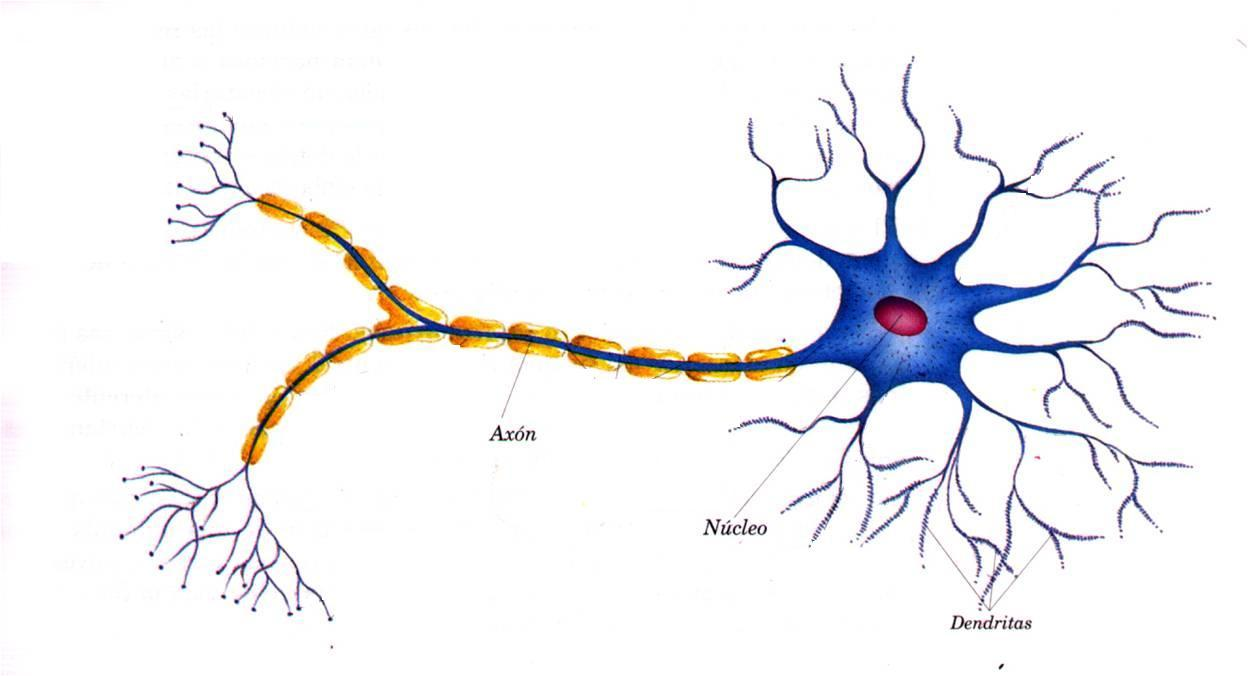
\includegraphics[width=\textwidth]{imag/neurona.jpg}
  \end{center}
\end{frame}

\begin{frame}
  \frametitle{Sinapsis}
  \begin{itemize}
  \item Cuando un impulso electrico viaja a través de un axón a una sinápsis, se transmite
    a través de un líquido neurotransmisor.
  \item El impulso se transmite por difusión a las neuronas receptoras.
  \item La efectividad de las sinápsis puede ser cambiada (peso sináptico).
  \item La sinápsis es lenta, pero usa muy poca energía, y se adapta a partir de señales disponibles localmente.
  \end{itemize}
\end{frame}

\begin{frame}
  \frametitle{¿Como funciona el cerebro?}
  \begin{itemize}
  \item Solo unas pocas neuronas se conectan con receptores o actuadores.
  \item Cada neurona recibe estimulos de otras neuronas.
  \item El efecto de cada entrada de otra neurona es controlado por
    un peso sináptico.
  \item El peso sináptico se adapta de forma que la red en forma global
    aprende a realizar operaciones útiles.
  \item Tenemos aproximadamente $10^{11}$ neuronas, cada una con $10^4$ pesos sinápticos.
  \end{itemize}
\end{frame}

\begin{frame}
  \frametitle{Modularidad del cerebro}
  \begin{center}
    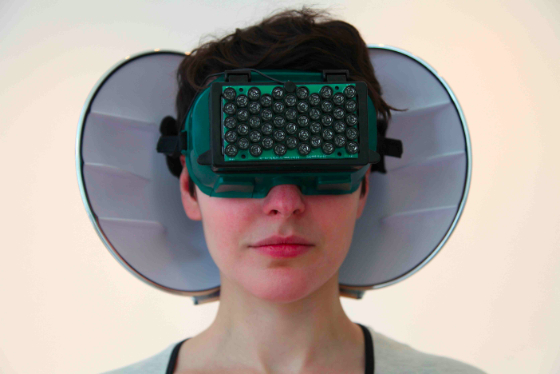
\includegraphics[width=0.9\textwidth]{imag/echo.jpg}
  \end{center}

\end{frame}

\begin{frame}
  \frametitle{Modularidad del cerebro}
  \begin{center}
    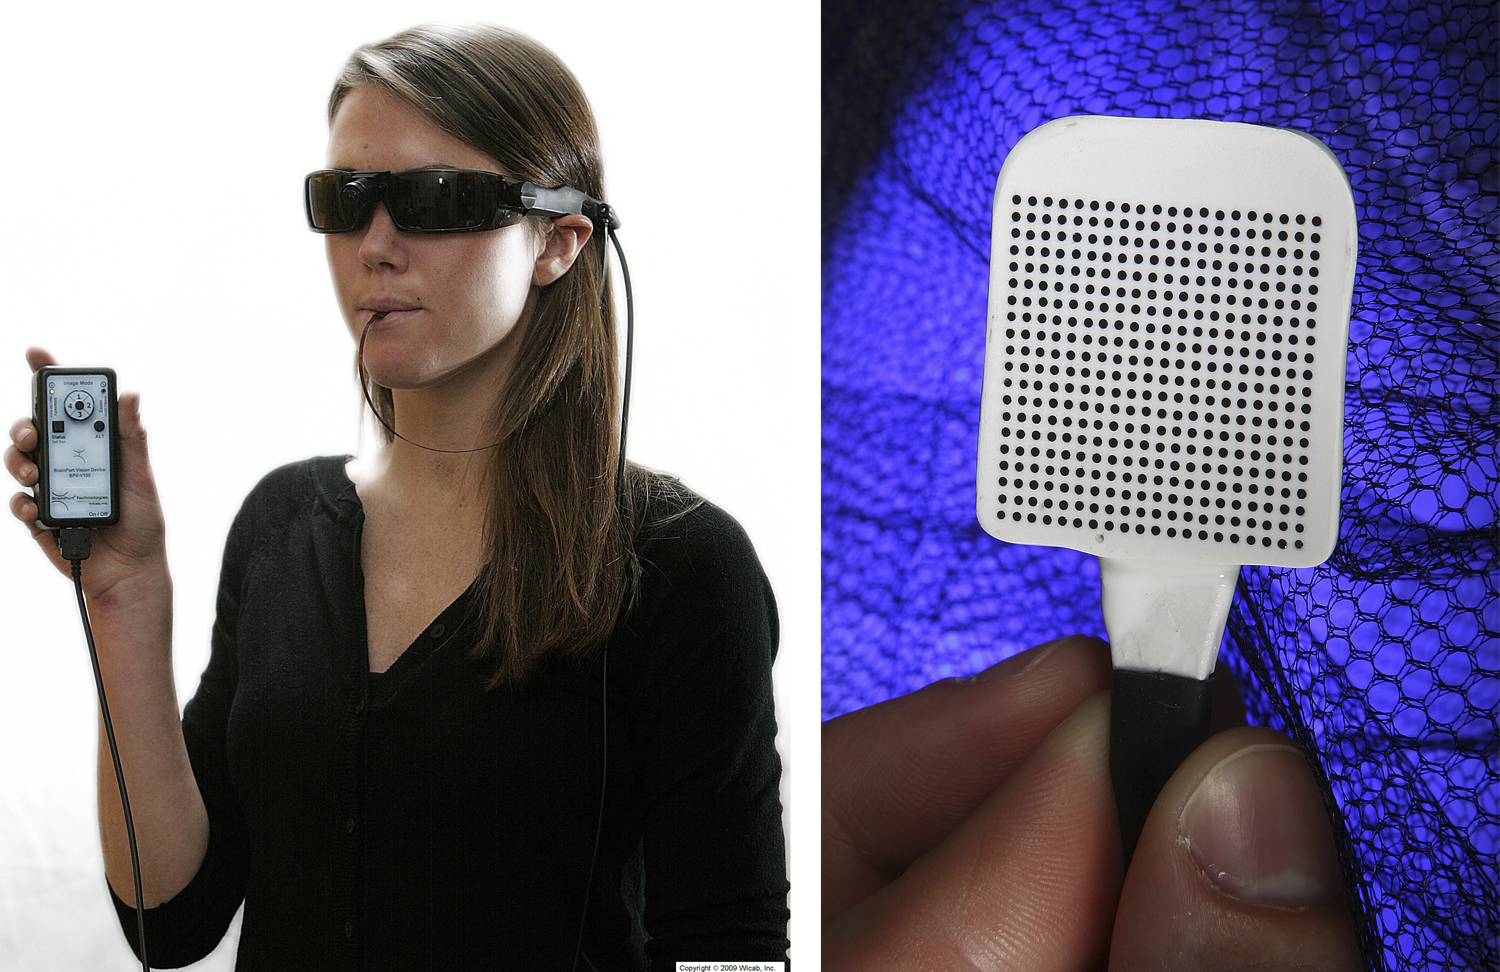
\includegraphics[width=\textwidth]{imag/ver_lengua.jpg}
  \end{center}
\end{frame}



\section{Modelos simples de una neurona}

\begin{frame}
  \frametitle{Modelos simples de una neurona}
  \begin{itemize}
  \item Para modelar cosas hay que idealizarlas.
  \item Eliminar detalles complicados no esenciales para la
    comprensión del fenómeno.
  \item Vale la pena realizar modelos comprensibles de cosas que
    sabemos son incorrectas (sin olvidar que son incorrectas).
  \item Asumamos que las neuronas transmiten valores reales y no
    impulsos.
  \end{itemize}
\end{frame}

\begin{frame}
  \frametitle{Neuronas lineales}
  \begin{block}{}
    $$ y = b + \sum_{i} \omega_i x_i$$
  \end{block}
  \begin{itemize}
  \item Si hacemos aprender a esta neurona, podemos probar con
    neuronas más complicadas.
  \item $y$ es la \alert{salida}, $b$ es el \alert{sesgo}, $x_i$ la $i$--ésima
    \alert{entrada} y $\omega_i$ el \alert{peso} en la $i$--ésima entrada.
  \end{itemize}
\end{frame}

\begin{frame}
  \frametitle{Neuronas binarias}
  \begin{block}{}
      $$ z = \sum_{i} \omega_i x_i $$
      $$ y = \left\{
          \begin{array}{ll}
            1 & \text{si}\ z \ge \theta \\
            0 & \text{en otro caso}
          \end{array} \right. $$
  \end{block}

  \begin{itemize}
  \item Propuestas por McCulloch y Pitts en 1943.
  \item Se asume que cada impulso es como el valor de verdad de una
    proposición lógica.
  \item El parámetro $\theta$ es un umbral.
  \end{itemize}
\end{frame}

\begin{frame}
  \frametitle{Neuronas binarias}

  \frametitle{Neuronas binarias}
  \begin{block}{Representación alternativa}
      $$ z = b + \sum_{i} \omega_i x_i$$
      $$ y = \left\{
          \begin{array}{ll}
            1 & \text{si}\ z \ge 0 \\
            0 & \text{en otro caso}
          \end{array} \right. $$
  \end{block}

  \begin{itemize}
  \item La neurona binaria es equivalente a aplicar una función no
    lineal a la neurona lineal.
  \item A esta función no lineal se le conoce como \alert{función de activación}
  \end{itemize}
\end{frame}

\begin{frame}
 \frametitle{Neuronas lineales rectificadas}
  \begin{block}{ReLU}
      $$ z = b + \sum_{i} \omega_i x_i$$
      $$ y = \left\{
          \begin{array}{ll}
            z & \text{si}\ z \ge 0 \\
            0 & \text{en otro caso}
          \end{array} \right. $$
  \end{block}

  \begin{itemize}
  \item Relativamente reciente, muy rápido de calcular.
  \item Muy eficiente en problemas de aprendizaje profundo.
  \end{itemize}
\end{frame}


\begin{frame}
 \frametitle{Neuronas sigmoidales}
  \begin{block}{Logística}
      $$ z = b + \sum_{i} \omega_i x_i$$
      $$ y = \frac{1}{1 + e^{-z}}$$
  \end{block}

  \begin{itemize}
  \item Devuelve un valor real acotado, imitando una neurona binaria.
  \item Fácil de derivar (lo que es útil para el aprendizaje).
  \item Las más usadas en modelos de pequeña y mediana escala.
  \end{itemize}
\end{frame}

\begin{frame}
 \frametitle{Neuronas estocásticas}
  \begin{block}{Estocástica}
      $$ z = b + \sum_{i} \omega_i x_i$$
      $$ P[s=1] = \frac{1}{1 + e^{-z}}$$
  \end{block}

  \begin{itemize}
  \item Mismas ecuaciones que la logística, pero diferente significado.
  \item Probabilidad de tener un impulso en un intervalo de tiempo corto.
  \item La salida es una V.A. con una distribución de Poisson.
  \end{itemize}
\end{frame}




\section{Arquitecturas principales}

\begin{frame}
  \frametitle{Arquitecturas principales de redes neuronales}
  \begin{itemize}
  \item Por arquitectura, consideramos la forma en que se conectan las
    neuronas entre si. Tambien se le conoce como \alert{topología} de
    la red neuronal.
  \item Dos arquitecturas generales básicas: \emph{alimentación hacia
      adelante}, y \emph{recursivas}.
  \item Para este curso nos centraremos en las de alimentación hacia adelante.
  \end{itemize}
\end{frame}

\begin{frame}
  \frametitle{Redes con alimentación hacia adelante}
  \begin{itemize}
  \item Redes más comunes en aplicaciones prácticas
  \item La primer capa es la entrada y la última la salida
  \item Si tienen más de una capa oculta se les conoce como redes
    neuronales \alert{profundas} (\emph{Deep neural network}).
  \item Calculan una serie de transformaciones de los datos de
    entrada.
  \item La función de activación de cada neurona es no lineal.
  \end{itemize}
\end{frame}

\begin{frame}
  \frametitle{Redes con alimentación hacia adelante}
  \begin{center}
    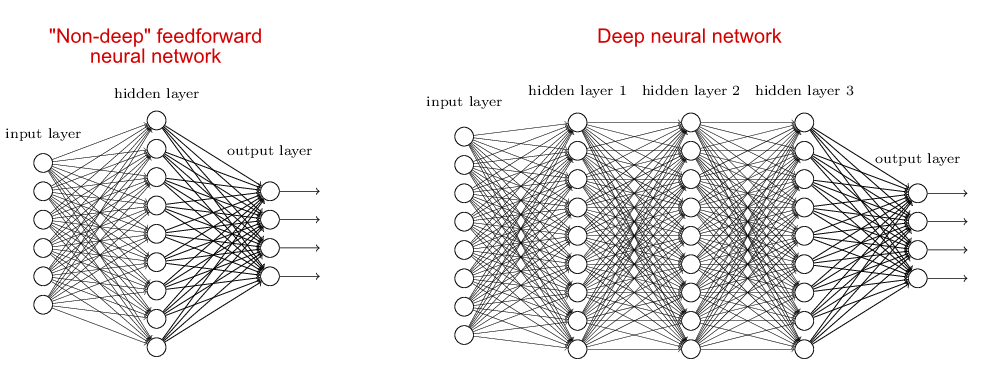
\includegraphics[width= \textwidth]{imag/feedforward.png}
  \end{center}
\end{frame}

\begin{frame}
  \frametitle{Redes recurrentes}
  \begin{itemize}
  \item Existen ciclos en sus conexiones
  \item Solo se pueden analizar en función del tiempo
  \item Dinámicas complicadas y dificultad en el aprendizaje
  \item Biológicamente son un poco más realistas
  \end{itemize}
\end{frame}

\begin{frame}
  \frametitle{Redes recurrentes}
  \begin{center}
    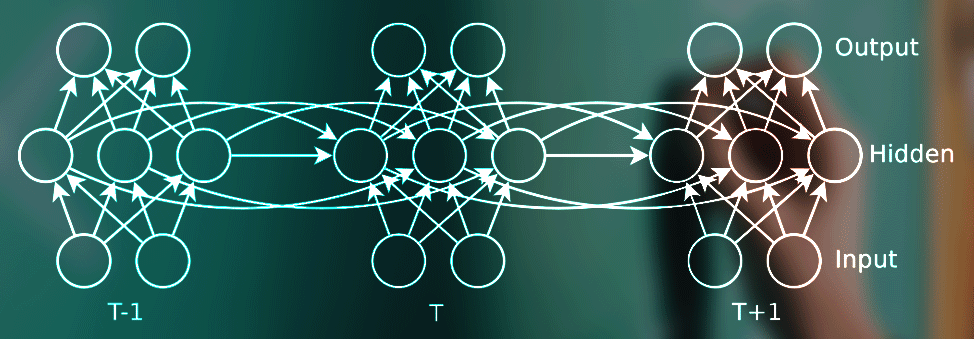
\includegraphics[width=\textwidth]{imag/recurrent.png}
  \end{center}
\end{frame}

\begin{frame}
  \frametitle{Aplicación de la redes recurrentes}
  \begin{itemize}
  \item Método natural para modelar información en forma secuencial
  \item Habilidad para recordar información
  \end{itemize}
  \begin{block}{Ejemplo (Fernando Alexis Martínez Valenzuela, 2017)}
    señores de la vida como razón de la plaza de sangrese favor de la
    integridad en el servicio público y el combate a la corrupción. se
    queó el gobierno ha querido subrayar hoy la armonía constitucional
    en que las inicias nuestra democracia, de la globalidad y del
    conocimiento. tenemos todo. tenemos el gran potencial para que
    cada mexicano escriba su propia historia de éxito. la correalidad
    de la falta de empleo, que no se otraín someterla afirarse para el
    desgreño, ausente de seriemos de corrupción.
  \end{block}
\end{frame}

\begin{frame}
  \frametitle{Redes recurrentes simétricas}

  \begin{itemize}
  \item Redes recurrentes, donde todas las conexiones son en ambas
    direcciones y con el mismo peso en ambas direcciones.
  \item Un caso \emph{simple} de analizar de redes recurrentes.
  \item Si no hay unidades ocultas se conocen como \alert{redes de
      Hopfield}.
  \item Si tiene unidades ocultas se conocen como \alert{máquinas de
      Boltzmann}.
  \end{itemize}
\end{frame}

\section{El perceptrón}

\begin{frame}
  \frametitle{El perceptrón}
  \begin{block}{}
    Y ahora regresemos a la más simple de las redes neuronales hacia
    adelante: \alert{El perceptrón}
  \end{block}

\begin{itemize}
\item Red neuronal hacia adelante, con solo dos capas (no hay capa
  oculta)
\item Las neuronas se modelan como \emph{neuronas binarias}
\end{itemize}

\end{frame}

\begin{frame}
  \frametitle{El Perceptrón}
  \begin{itemize}
  \item Popularizado por Rosenblatt a principios de los 60.
  \item Parecían tener gran poder de aprendizaje en la época.
  \item En 1969, Minsky y Papert hacen pedazos al perceptrón.
  \item Actualmente es usado en problemas con varios millones de
    entradas.
  \end{itemize}
\end{frame}

\section{Un ejemplo simple de aprendizaje del perceptrón}

\begin{frame}
  \frametitle{Ejemplo simple de un perceptrón}

  \begin{itemize}
  \item Red simple para reconocer formas escritas a mano.
  \item Dos capas de neuronas:
    \begin{itemize}
    \item Neuronas en la primer capa representan intensidad de
      pixeles.
    \item Neuronas en la segunda capa representan formas conocidas.
    \end{itemize}
  \item Un pixel vota por una forma solo si tiene tinta.
  \item Cada pixel puede vota por cada forma.
  \item La forma más votada es seleccionada.
  \end{itemize}

\end{frame}

\begin{frame}
  \frametitle{Ilustración del problema}
  \begin{center}
    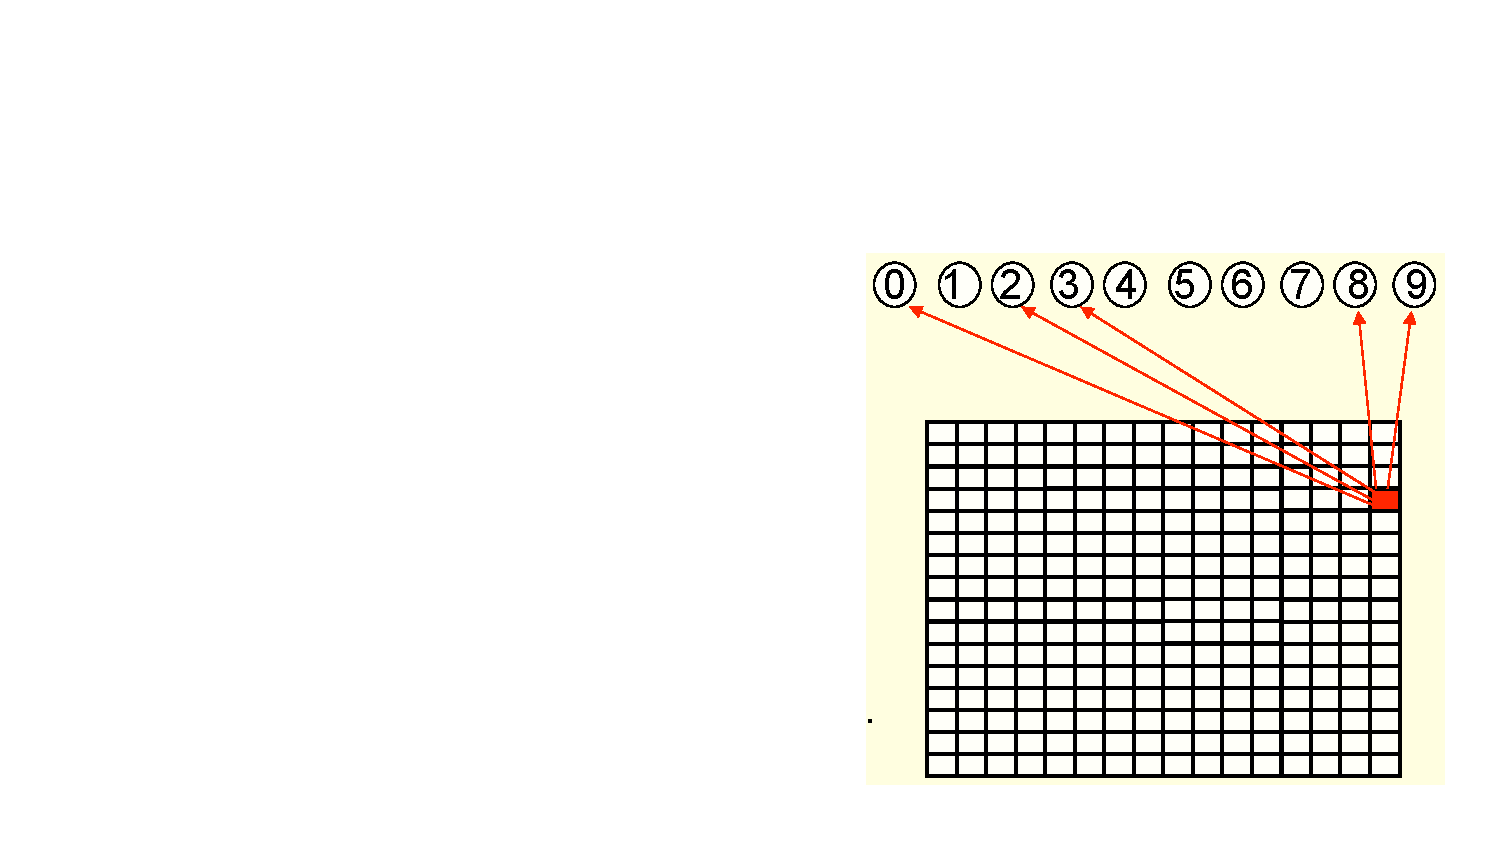
\includegraphics[width=.7\textwidth]{imag/ejemplo_0.pdf}
  \end{center}
\end{frame}

\begin{frame}
  \frametitle{Representación de pesos}
   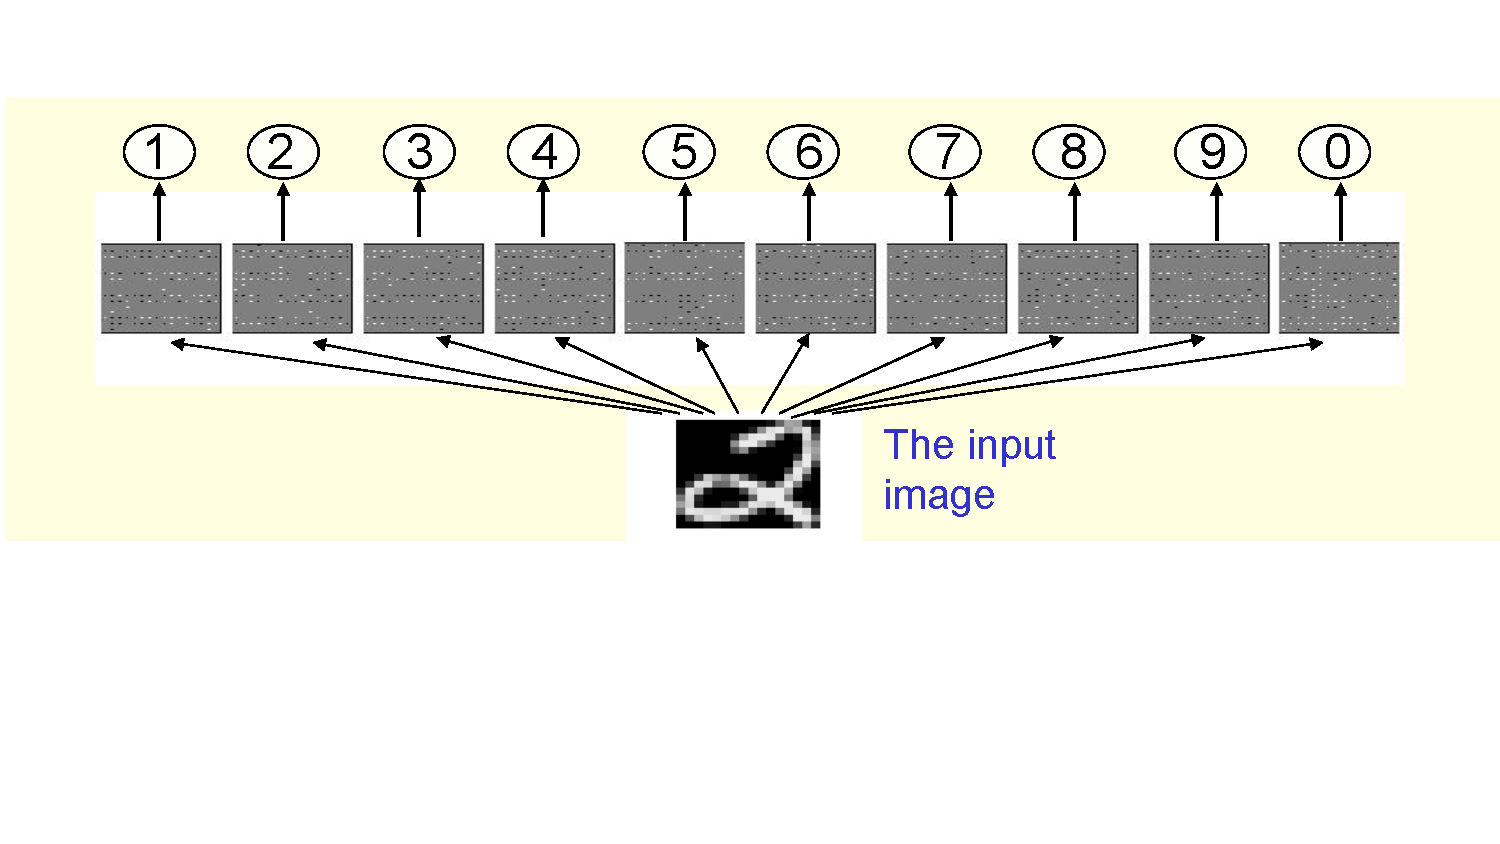
\includegraphics[width=\textwidth]{imag/ejemplo_1.pdf}

   \begin{itemize}
   \item El color (blanco o negro) representa el signo del voto.
   \item El área representa la intensidad (peso) del voto.
   \end{itemize}
\end{frame}

\begin{frame}
  \frametitle{Aprendizaje}
   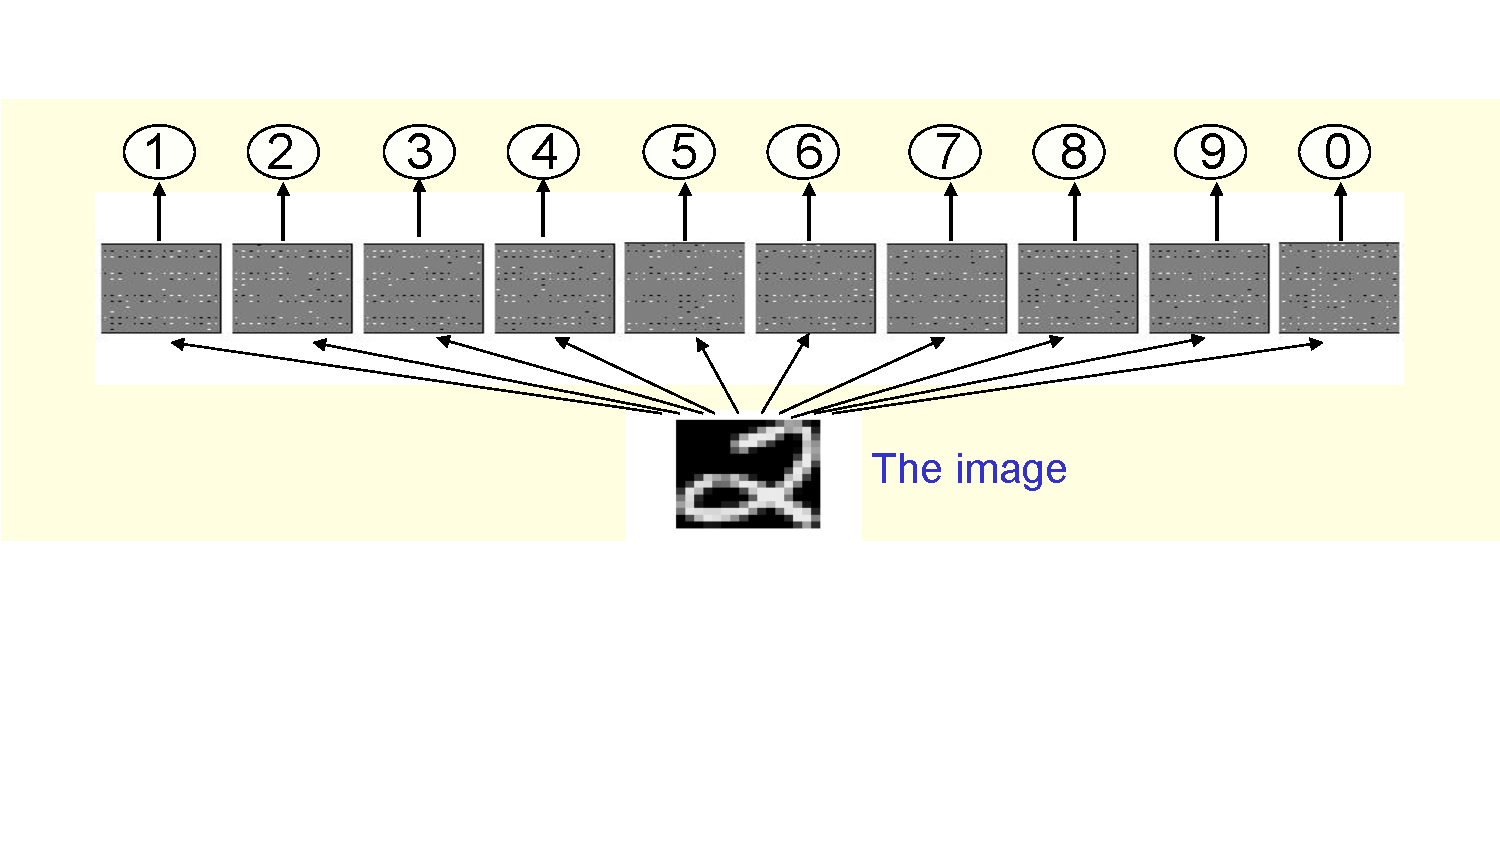
\includegraphics[width=\textwidth]{imag/ejemplo_2.pdf}

   \begin{itemize}
   \item Muestra un ejemplo conocido a la red, e incrementa el peso de
     los pixeles activos para la forma correcta.
   \item Decrementa el peso de los pixeles activos para la forma
     seleccionada por la red neuronal.
   \end{itemize}
\end{frame}

\begin{frame}
  \frametitle{Aprendizaje}
   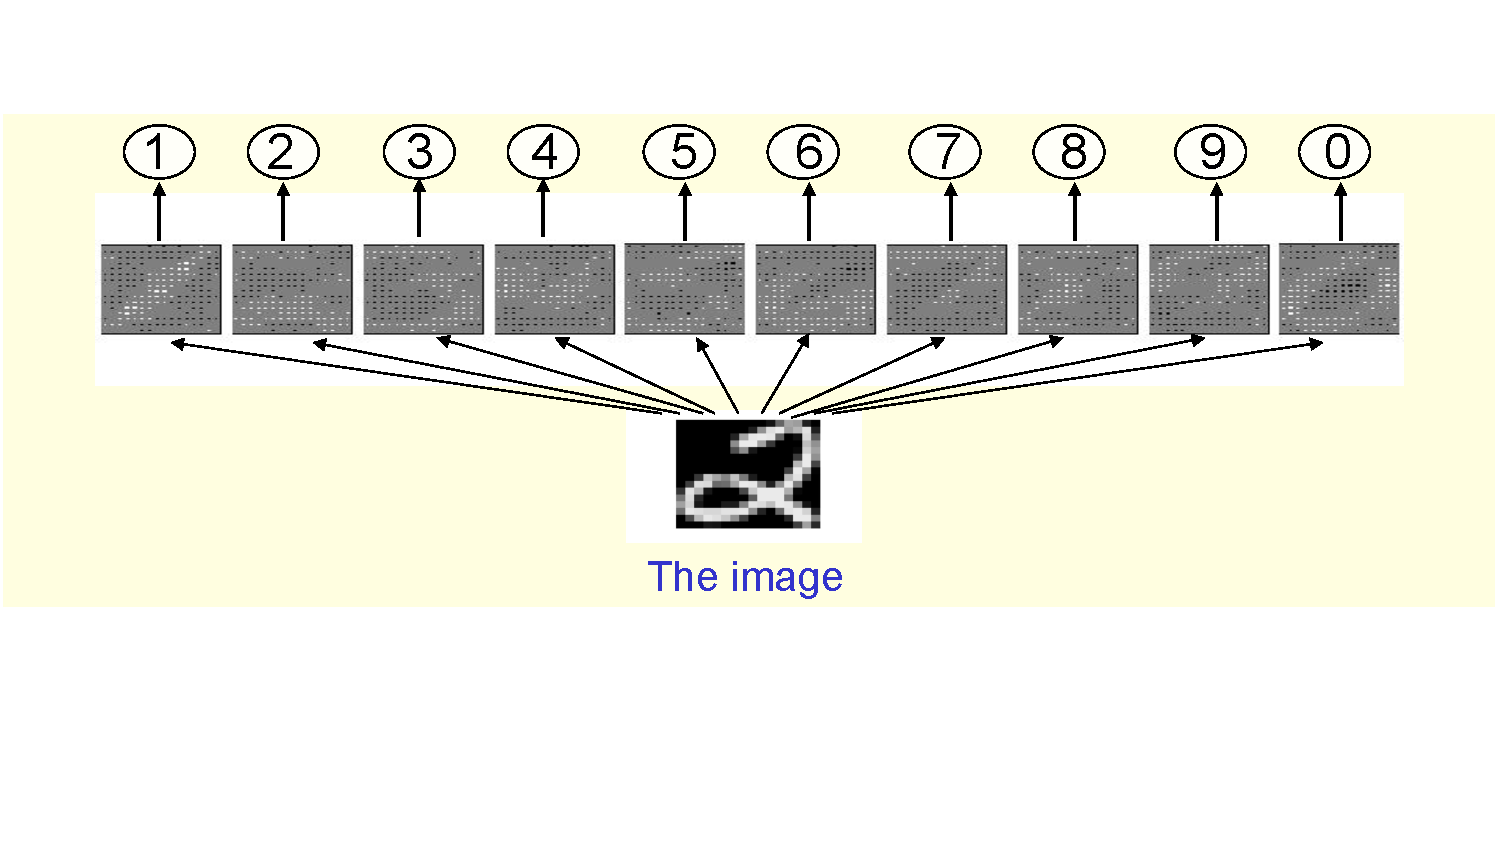
\includegraphics[width=\textwidth]{imag/ejemplo_3.pdf}
\end{frame}

\begin{frame}
  \frametitle{Aprendizaje}
   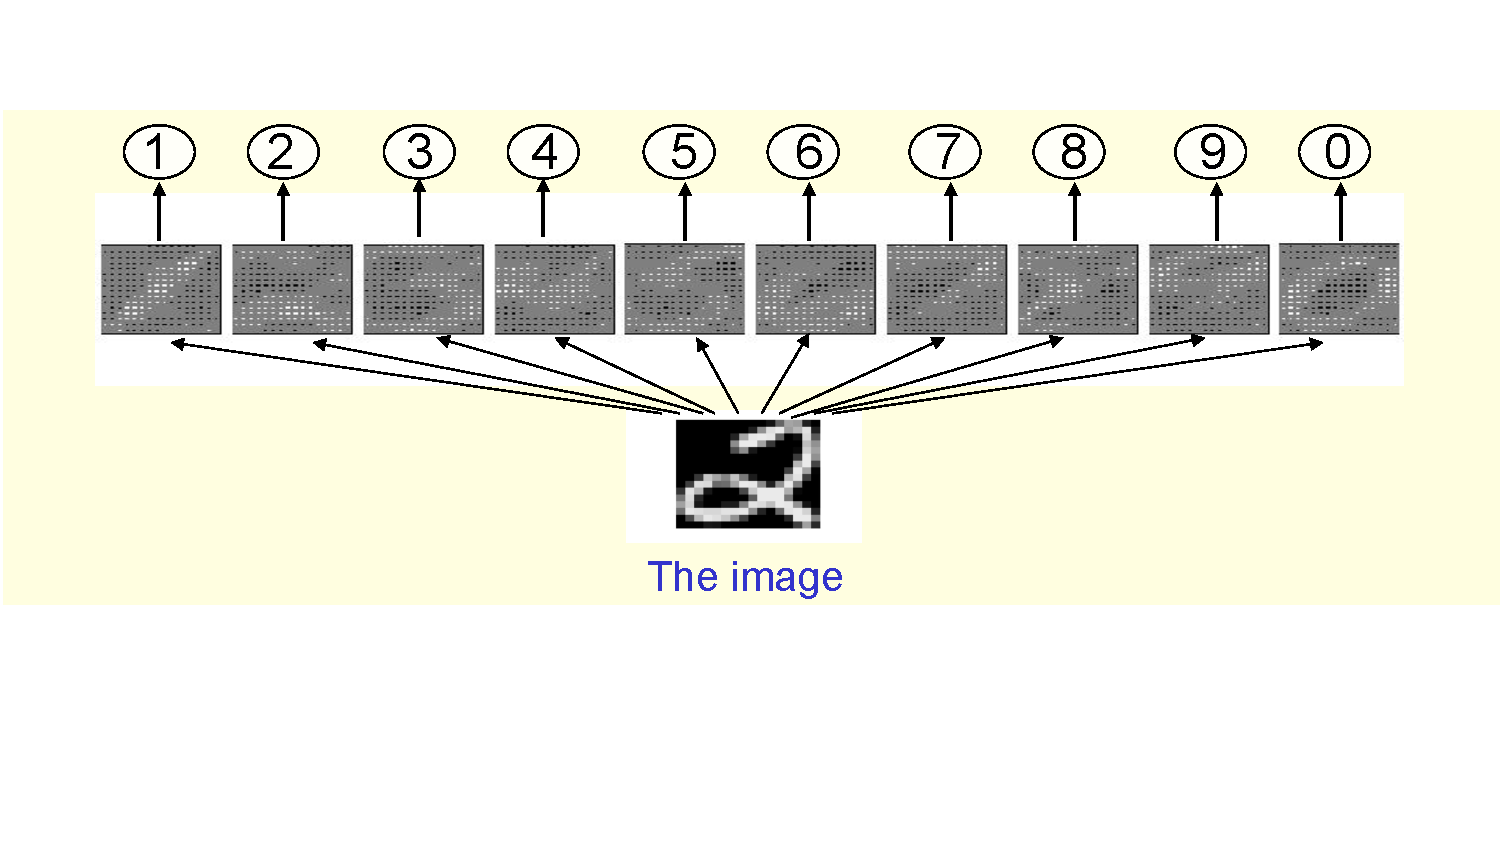
\includegraphics[width=\textwidth]{imag/ejemplo_4.pdf}
\end{frame}

\begin{frame}
  \frametitle{Aprendizaje}
   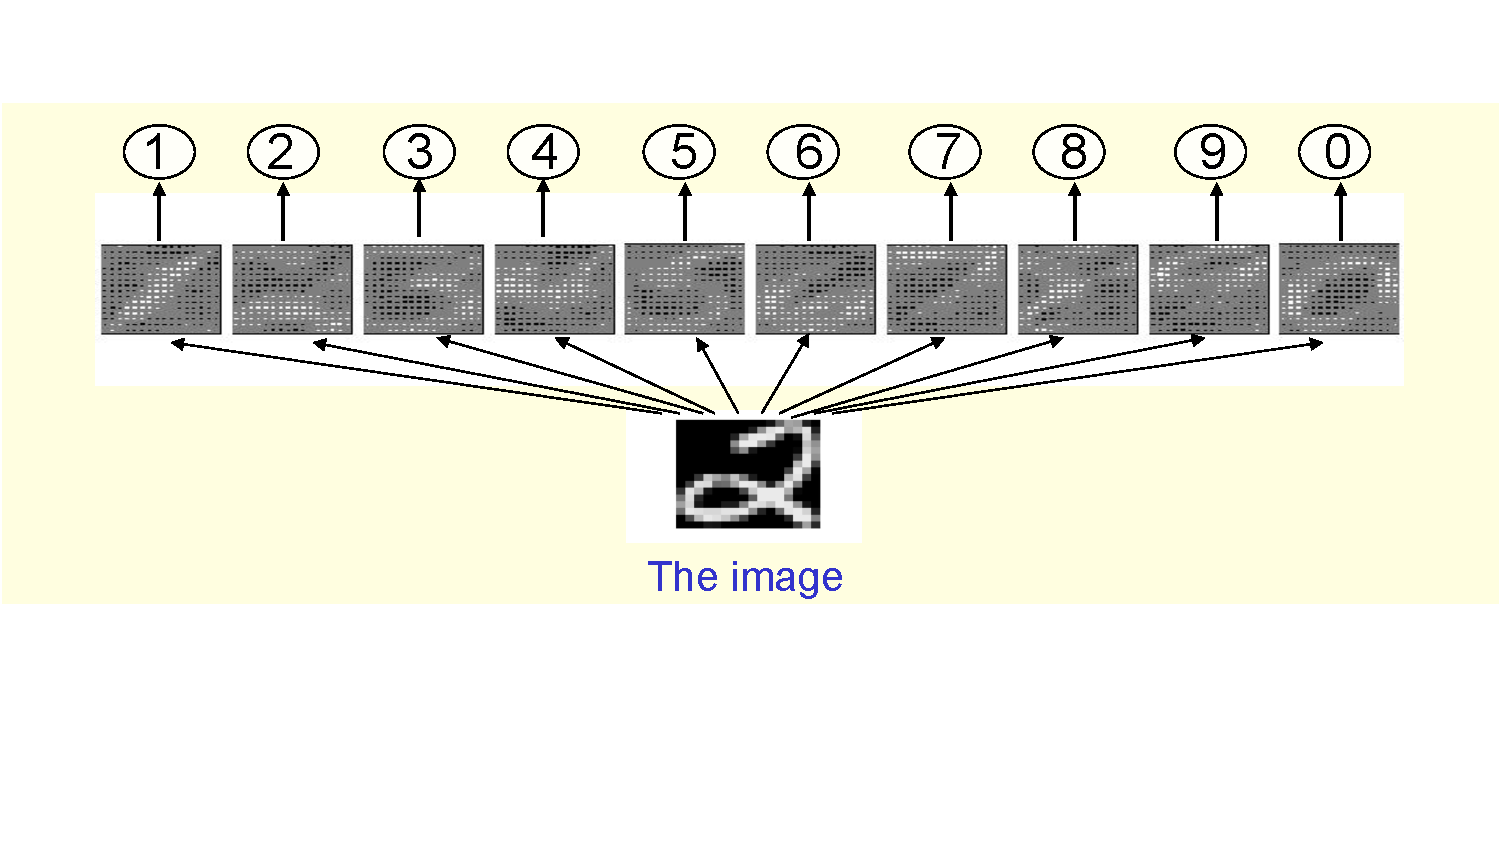
\includegraphics[width=\textwidth]{imag/ejemplo_5.pdf}
\end{frame}

\begin{frame}
  \frametitle{Aprendizaje}
   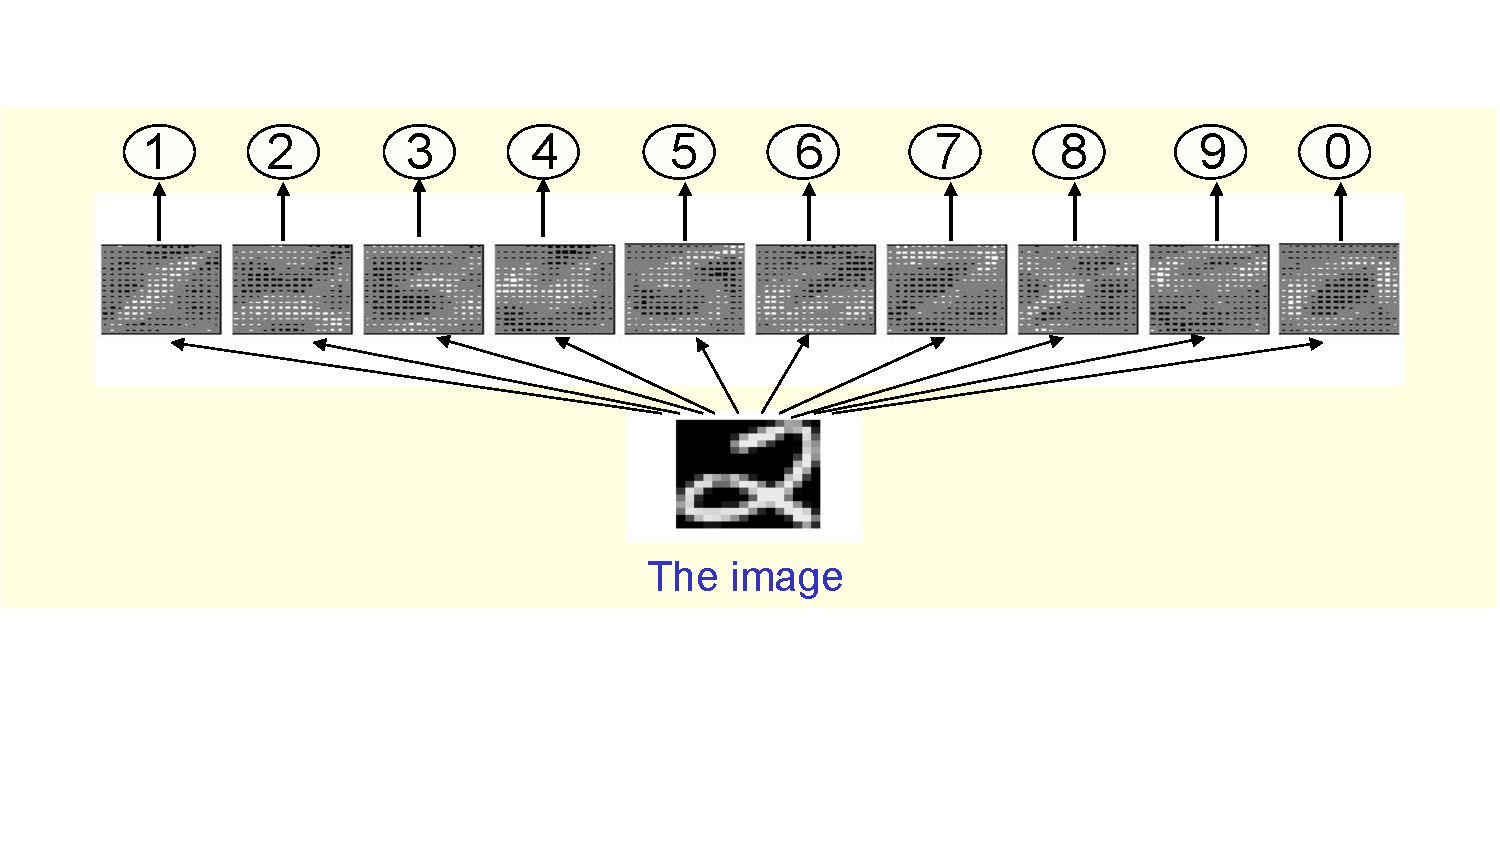
\includegraphics[width=\textwidth]{imag/ejemplo_6.pdf}
\end{frame}

\begin{frame}
  \frametitle{Aprendizaje}
   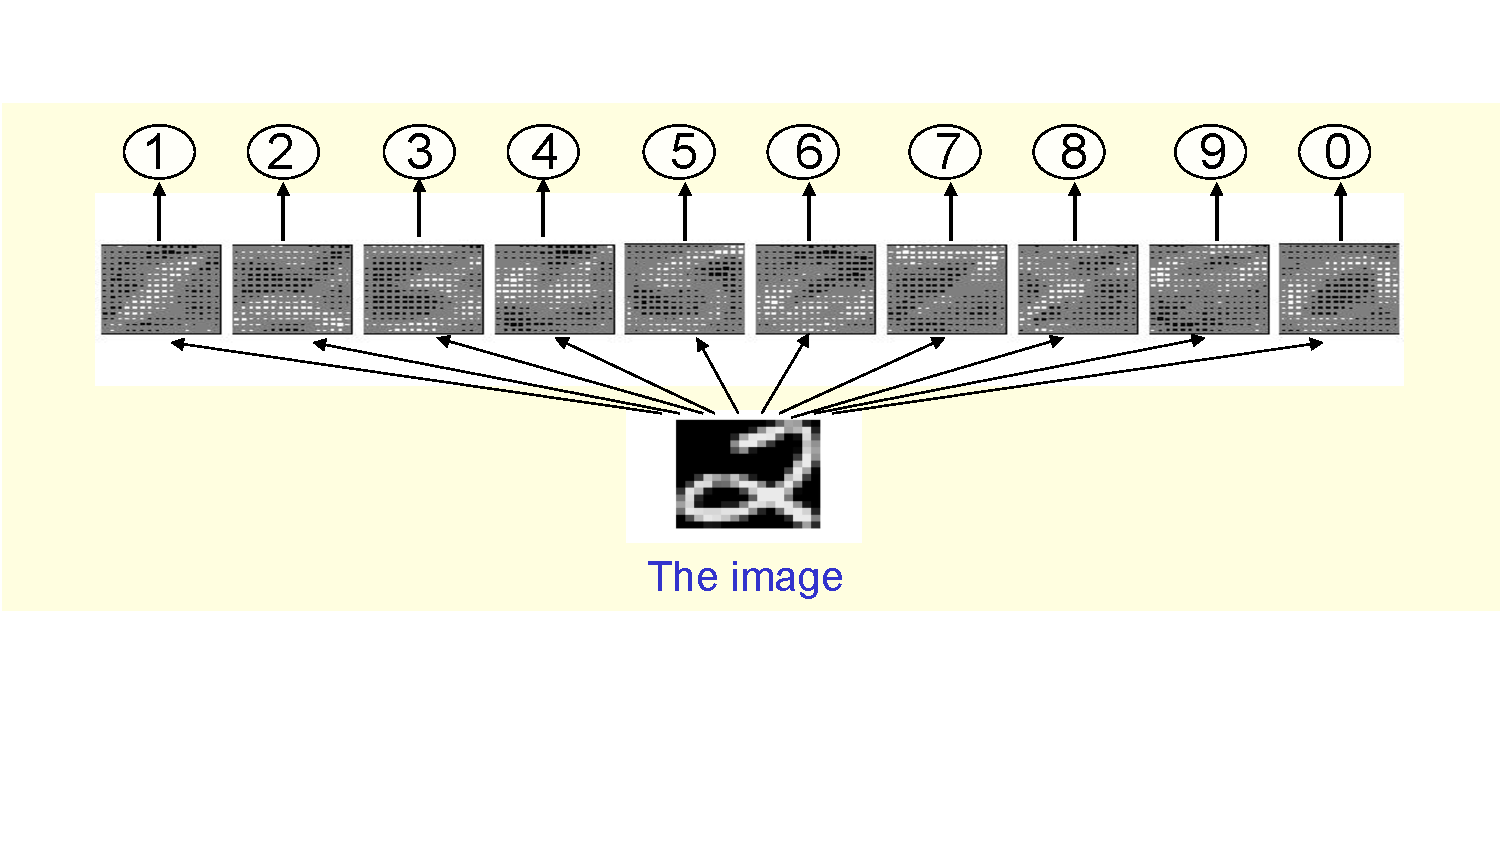
\includegraphics[width=\textwidth]{imag/ejemplo_7.pdf}
\end{frame}

\begin{frame}
  \frametitle{Aprendizaje}
   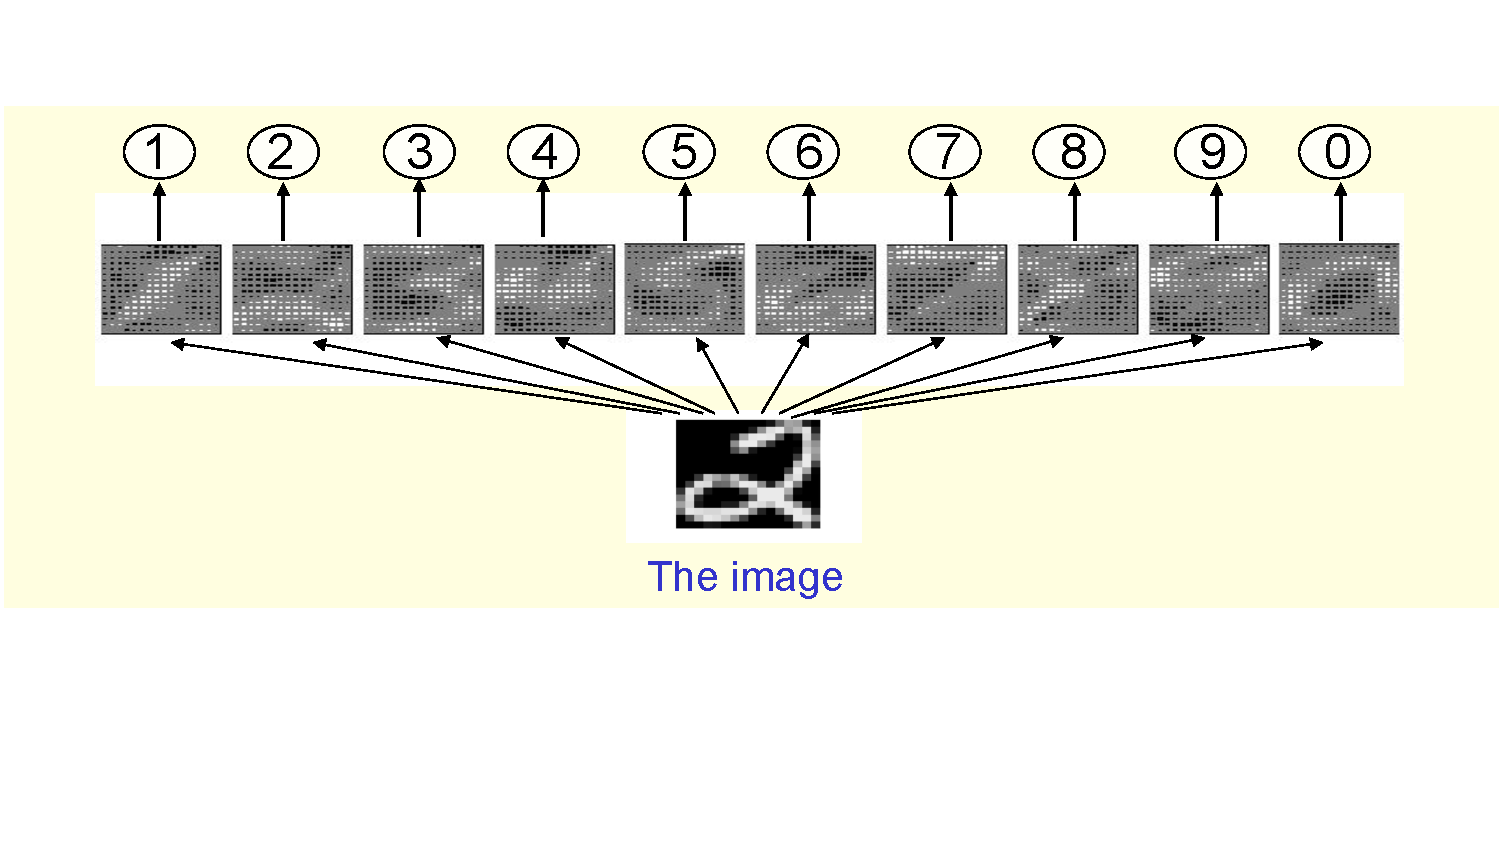
\includegraphics[width=\textwidth]{imag/ejemplo_8.pdf}
\end{frame}

\begin{frame}
  \frametitle{Problemas con el aprendizaje}

  \begin{itemize}
  \item Una red con solo dos capas es equivalente a un
    patron rígido por cada forma.
  \item El ganador es el patron con más traslape.
  \item Los dígitos escritos a mano son mucho más complejos.
  \item Es necesario capturar otras características.
  \end{itemize}
\end{frame}

\begin{frame}
  \frametitle{Ejemplo de dígitos escritos a mano}
  \begin{center}
    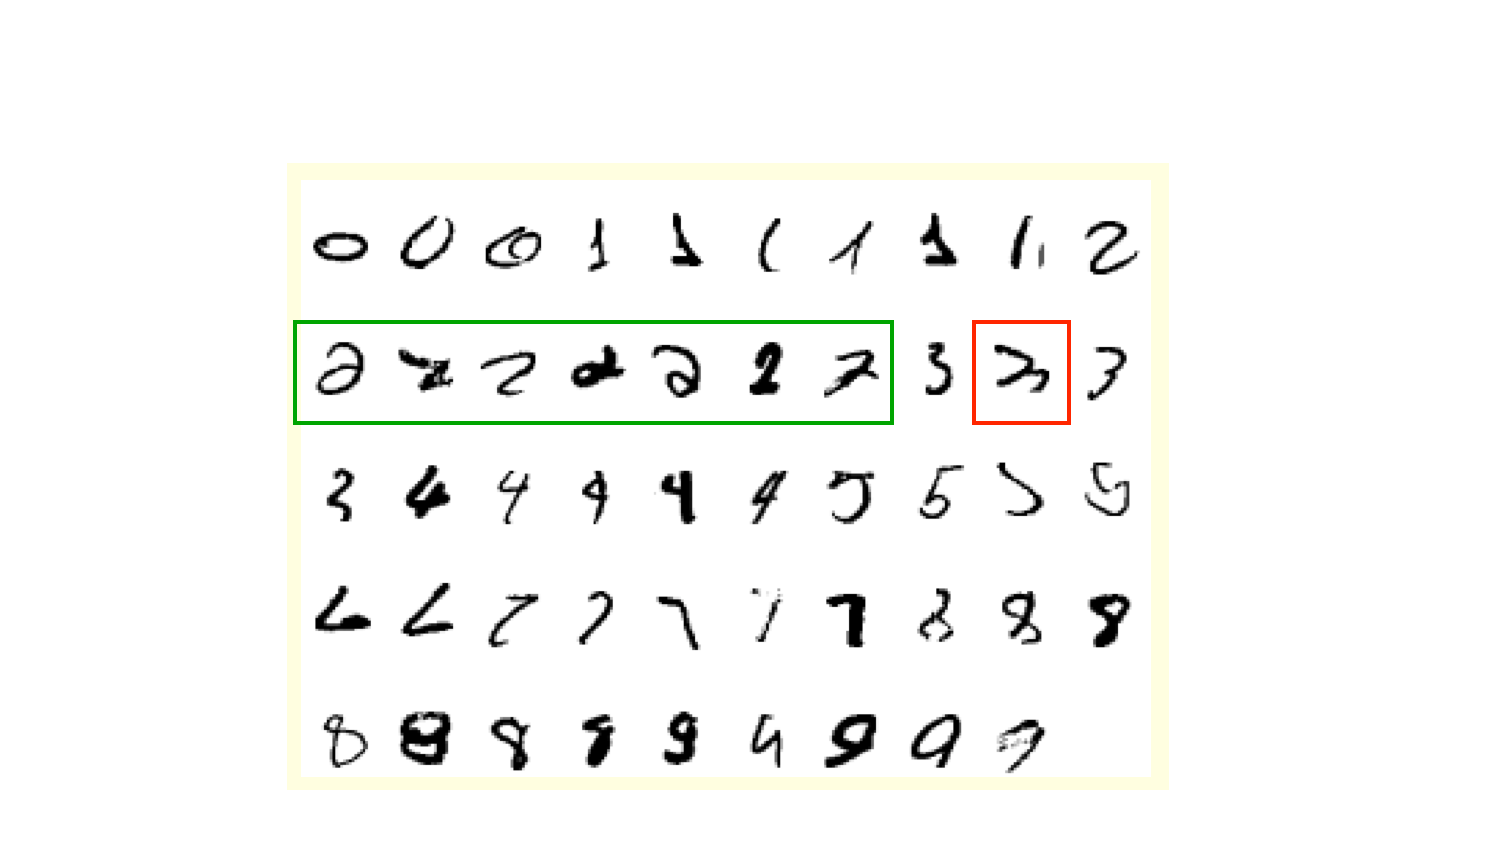
\includegraphics[width=0.8\textwidth]{imag/ejemplo_9.pdf}
  \end{center}
\end{frame}

\begin{frame}
  \frametitle{Limitaciones del perceptrón}
El perceptrón no puede resolver ni siquiera los problemas más
elementales no linealmente separables.
  \begin{center}
    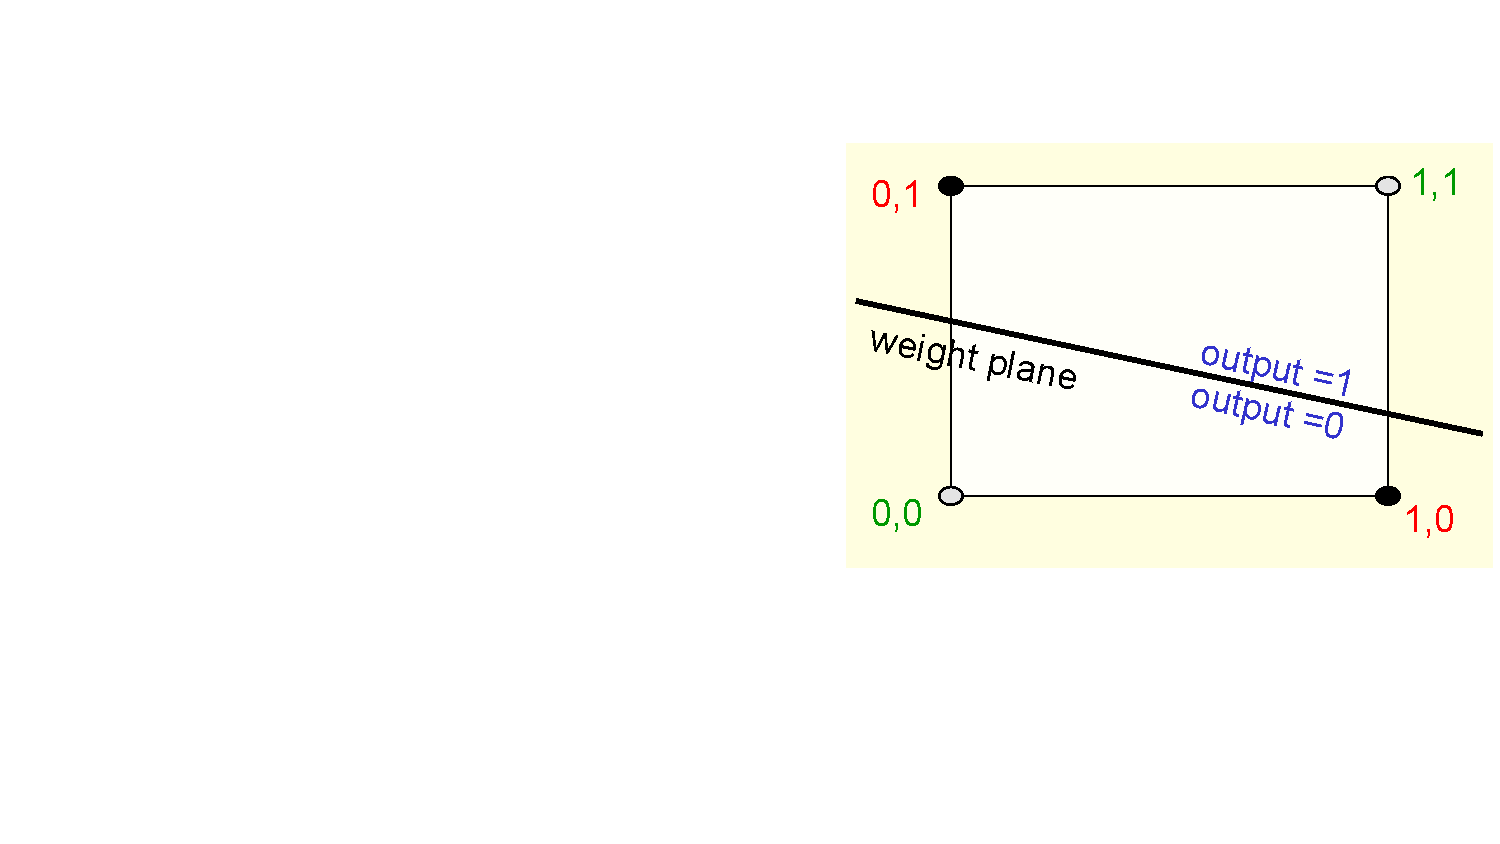
\includegraphics[width=0.8\textwidth]{imag/xor_perceptron.pdf}
  \end{center}

\end{frame}

\begin{frame}
  \frametitle{Limitaciones del perceptrón}
El perceptrón no puede resolver patrones simples con translación.
  \begin{center}
    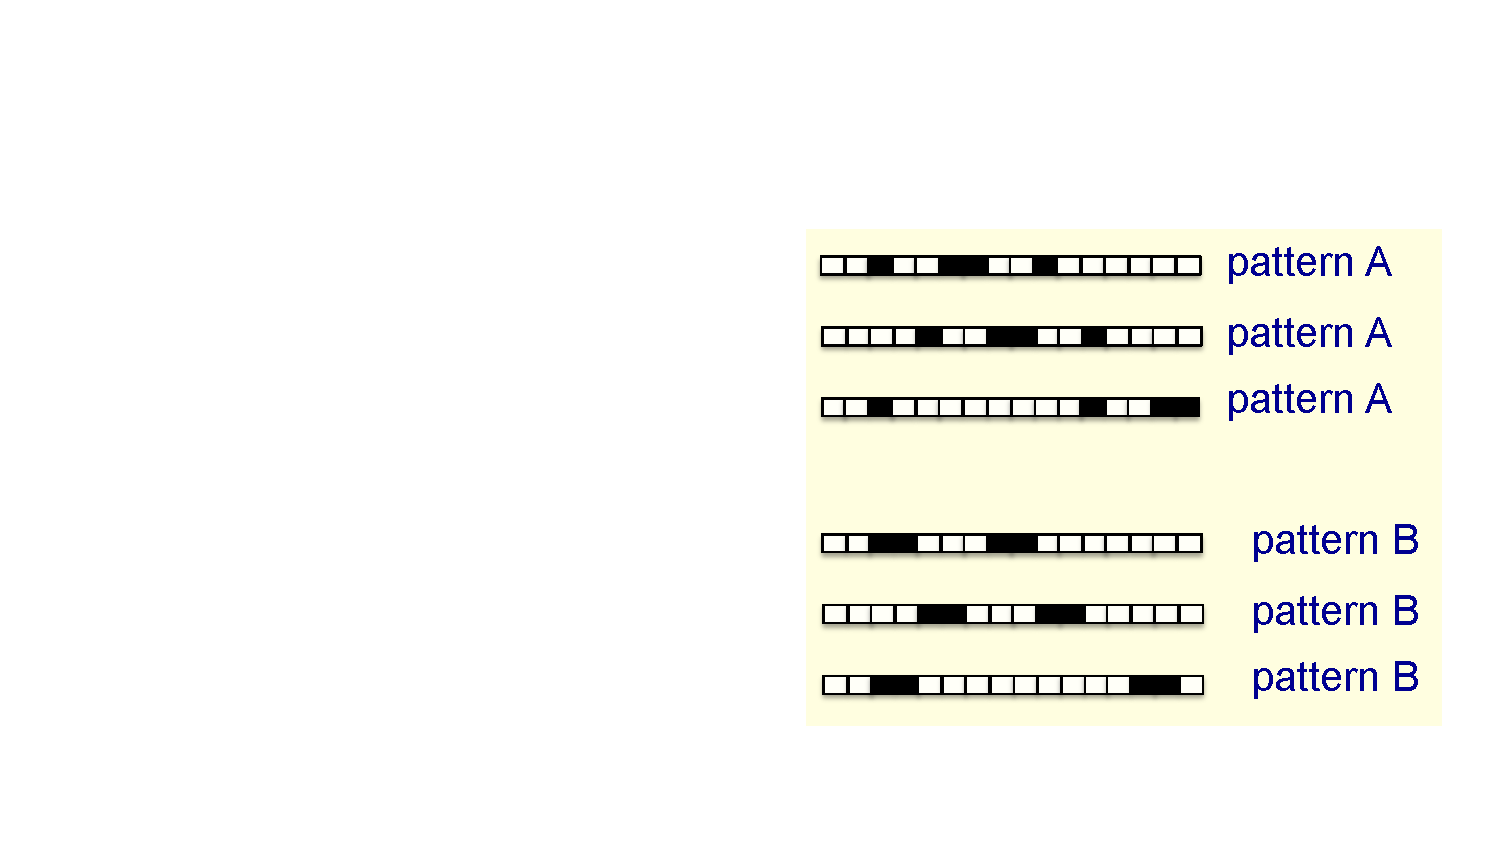
\includegraphics[width=0.7\textwidth]{imag/tanslacion_perceptron.pdf}
  \end{center}

\end{frame}

\begin{frame}
  \frametitle{Una catastrofe para las redes neuronales}
  \begin{itemize}
  \item El objetivo del reconocimiento de patrones es reconocer
    patrones, a pesar de transformaciones como la translación.
  \item Para resolver estos problemas, es necesario extraer otro tipo
    de características para reconocer translaciones, u otro subpatron
    informativo.
  \item La parte sabrosa entonces hay que programarla a mano, y le
    dejamos el problema fácil al algoritmo de aprendizaje.
  \end{itemize}
\end{frame}

\begin{frame}
  \frametitle{Aprendizaje con neuronas ocultas}

  \begin{itemize}
  \item Redes sin neuronas ocultas solo pueden hacer funciones muy
    simples entre las entradas y las salidas.
    \begin{itemize}
    \item Neuronas ocultas lineales no ayudan, el resultado sigue
      siendo una combinación lineal de las entradas.
    \item No linealidades fijas a la salida tampoco son suficientes.
    \end{itemize}
  \item Es necesario agregar capas de neuronas adaptables y no
    lineales.
    \begin{itemize}
    \item Para que esto sea posible es necesario ajustar \emph{todos}
      los pesos al mismo tiempo, y no solo los de la capa de salida.
    \item Aprender pesos en las capas ocultas es equivalente a
      aprender nuevas características.
    \item Problema difícil, ya que nadie da indicaciones de como deben
      ser esas nuevas características.
    \end{itemize}
  \end{itemize}

\end{frame}

\end{document}
